% ============================================================
%  第 3 章  积分变换：傅里叶分析与拉普拉斯变换（扩展版）
% ============================================================

\chapter{积分变换：傅里叶分析与拉普拉斯变换}

\section{本章概览与学习路线}

傅里叶变换和拉普拉斯变换是物理学家最重要的两种积分变换工具。它们将函数从时域（或空间域）映射到频域（或复频域），将微分方程转化为代数方程，将卷积转化为乘法。

\begin{center}
\fbox{\parbox{0.9\textwidth}{\centering
\textbf{核心逻辑链条：}\\
周期信号 $\to$ 傅里叶级数（离散谱）$\to$ 非周期信号 $\to$ 傅里叶变换（连续谱）\\
$\to$ 收敛性问题 $\to$ 拉普拉斯变换（复频域）$\to$ 传递函数与系统分析
}}
\end{center}

\subsection*{不同读者的学习路径}

\begin{itemize}
\item \textbf{物理专业学生：} 重点关注 \S3.3（FT 基本性质）、\S3.4（FT 物理应用——衍射、量子力学、不确定性原理）、\S3.5（Laplace 变换求解 ODE）、\S3.6（RLC 电路与传递函数）。
\item \textbf{信号处理/电子工程学生：} 重点关注 \S3.2（傅里叶级数的工程应用）、\S3.3（FT 性质与卷积定理）、\S3.4（采样定理、滤波器设计）、\S3.6（传递函数与稳定性）。
\item \textbf{数学学生：} 重点关注 FT 和 Laplace 变换的严格推导、收敛条件、逆变换的围道积分表示。
\end{itemize}

\section{傅里叶级数}
\label{sec:fourier_series}

\subsection*{动机：为什么周期运动可以分解为谐波？}

伽利略发现摆的周期与振幅无关（小角度下是简谐运动），傅里叶则做了相反的事：任何周期运动都可以看作多个不同频率简谐运动的叠加。这就是说：\textbf{简谐运动不是特例，而是周期运动的基本"砖块"}。

\subsection{周期函数的谐波分解}

设 $f(t)$ 是周期为 $T$ 的函数，在合适的正则条件下可以展开为傅里叶级数：
\begin{equation}
f(t) = \frac{a_0}{2} + \sum_{n=1}^{\infty}
\left[a_n\cos(n\omega_0 t) + b_n\sin(n\omega_0 t)\right],
\label{eq:fourier_series_tri}
\end{equation}
其中 $\omega_0 = 2\pi/T$ 是基频。傅里叶系数由正交性给出：
\begin{align}
a_n &= \frac{2}{T}\int_{-T/2}^{T/2} f(t)\cos(n\omega_0 t)\,\dd t,\\
b_n &= \frac{2}{T}\int_{-T/2}^{T/2} f(t)\sin(n\omega_0 t)\,\dd t.
\end{align}

\textbf{复数形式}（更适合理论分析）：
\begin{equation}
f(t) = \sum_{n=-\infty}^{\infty} c_n e^{\mathrm{i}n\omega_0 t},
\qquad
c_n = \frac{1}{T}\int_{-T/2}^{T/2} f(t)e^{-\mathrm{i}n\omega_0 t}\,\dd t.
\label{eq:fourier_series_complex}
\end{equation}

两种形式的关系：$c_0 = a_0/2$, $c_n = (a_n - \mathrm{i}b_n)/2$, $c_{-n} = (a_n + \mathrm{i}b_n)/2$（$n\geq1$）。

\subsection{收敛条件（Dirichlet 条件）}

傅里叶级数在以下条件下逐点收敛到 $f(t)$：
\begin{itemize}
\item $f(t)$ 在一个周期内绝对可积：$\int_{-T/2}^{T/2} |f(t)|\,\dd t < \infty$。
\item $f(t)$ 在一个周期内只有有限个极值点和有限个间断点。
\end{itemize}
在间断点处，傅里叶级数收敛到左右极限的平均值：$\frac{f(t_0^+) + f(t_0^-)}{2}$。

\begin{example}[方波的傅里叶级数]
周期为 $2\pi$ 的方波：
\begin{equation}
f(t) = \begin{cases}
1, & 0 < t < \pi,\\
-1, & -\pi < t < 0.
\end{cases}
\end{equation}

由于 $f(t)$ 是奇函数，$a_n=0$。计算 $b_n$：
\begin{align*}
b_n &= \frac{1}{\pi}\int_{-\pi}^{\pi} f(t)\sin(nt)\,\dd t
= \frac{2}{\pi}\int_{0}^{\pi} \sin(nt)\,\dd t \\
&= \frac{2}{\pi}\left[-\frac{\cos(nt)}{n}\right]_0^{\pi}
= \frac{2}{n\pi}(1 - \cos n\pi) \\
&= \begin{cases}
4/(n\pi), & n\text{ 奇数},\\
0, & n\text{ 偶数}.
\end{cases}
\end{align*}

因此方波的傅里叶级数为：
\begin{equation}
f(t) = \frac{4}{\pi}\sum_{k=0}^{\infty}\frac{\sin[(2k+1)t]}{2k+1}
= \frac{4}{\pi}\left(\sin t + \frac{1}{3}\sin 3t + \frac{1}{5}\sin 5t + \cdots\right).
\end{equation}
在跳跃点 $t=0,\pm\pi$ 处，级数收敛到 $0$——这正是左右极限的平均值 $(1+(-1))/2=0$。
\end{example}

\begin{example}[锯齿波的傅里叶级数]
周期为 $2\pi$ 的锯齿波：$f(t) = t$, $t\in(-\pi,\pi)$。

由于 $f(t)$ 是奇函数，$a_n=0$。
\begin{align*}
b_n &= \frac{1}{\pi}\int_{-\pi}^{\pi} t\sin(nt)\,\dd t
= \frac{2}{\pi}\int_{0}^{\pi} t\sin(nt)\,\dd t\quad(\text{奇函数}\times\text{奇函数}=\text{偶函数}) \\
&= \frac{2}{\pi}\left[\frac{\sin(nt) - nt\cos(nt)}{n^2}\right]_0^{\pi}
= \frac{2}{\pi}\cdot\frac{-\pi\cos(n\pi)}{n} = \frac{(-1)^{n+1}2}{n}.
\end{align*}

因此：
\begin{equation}
t = 2\sum_{n=1}^{\infty} \frac{(-1)^{n+1}}{n}\sin(nt),\qquad -\pi < t < \pi.
\end{equation}

在 $t=\pm\pi$ 处，级数收敛到 $0$，恰好是 $f(-\pi)$ 和 $f(\pi)$ 的平均值。
\end{example}

\begin{insight}[傅里叶级数的物理意义]
三角函数的正交性 $\int_0^T \cos(n\omega_0 t)\cos(m\omega_0 t)\,\dd t \propto \delta_{nm}$ 保证了这个分解的"唯一性"——每个频率成分是独立的自由度。在振动分析中，$|c_n|^2$ 正比于第 $n$ 阶谐波的能量。这解释了为什么拨动吉他的弦虽然产生的是基频的周期运动，但音色（谐波成分的比例）使不同乐器能够区分。
\end{insight}

% 傅里叶级数逼近图
\begin{figure}[H]
\centering
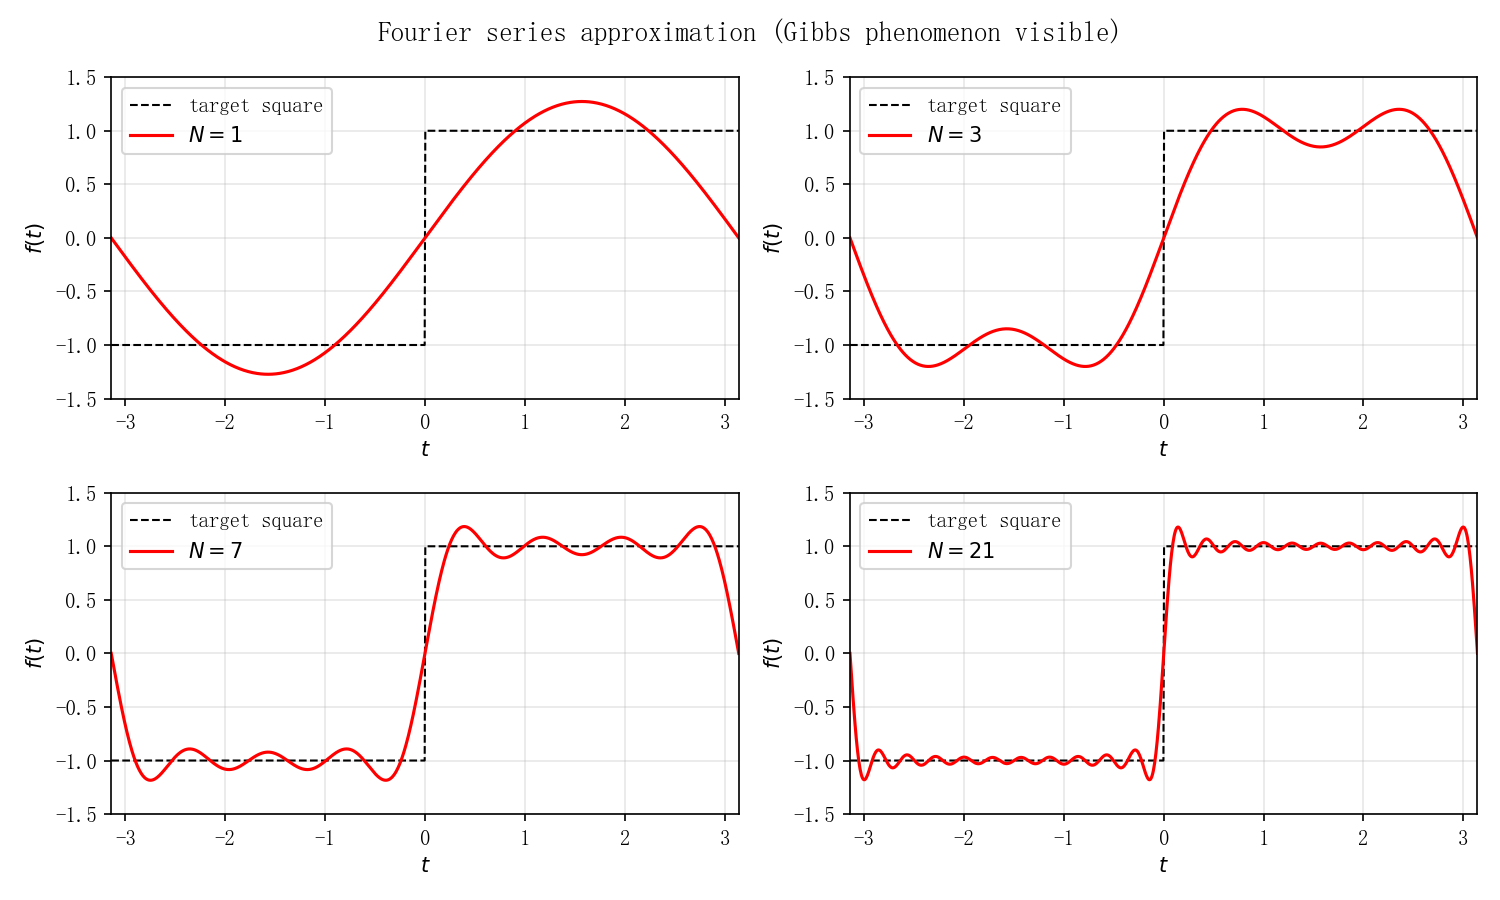
\includegraphics[width=0.8\textwidth]{figures/fig3_1_fourier_series.png}
\caption{傅里叶级数对方波的逼近。$N=1$ 仅含基频，$N=7$ 已较好地近似了方波形状。注意在跳跃点附近出现过冲（吉布斯现象），不随 $N$ 增加而消失。}
\label{fig:fourier_series}
\end{figure}

\subsection{吉布斯现象}

在函数的不连续点附近，傅里叶级数的部分和会出现过冲，这就是\textbf{吉布斯现象 (Gibbs phenomenon)}。过冲幅度约为跳跃高度的 $9\%$，且不随项数增加而消失——它只是越来越逼近跳跃点。

吉布斯现象在信号处理中至关重要：它告诉我们在用有限带宽近似陡峭边沿时，总会存在过冲和振铃。这也暗示了为什么需要在数字信号处理中使用窗函数（如 Hanning、Hamming 窗）来减轻这种效应。

\subsection{傅里叶级数的能量解释}

\textbf{帕塞瓦尔定理（傅里叶级数形式）：}
\begin{equation}
\frac{1}{T}\int_{-T/2}^{T/2} |f(t)|^2\,\dd t
= \frac{a_0^2}{4} + \frac{1}{2}\sum_{n=1}^{\infty}(a_n^2 + b_n^2)
= \sum_{n=-\infty}^{\infty} |c_n|^2.
\label{eq:parseval_series}
\end{equation}

物理意义：信号在一个周期内的平均功率等于各频率成分功率之和。这保证了时域和频域的能量守恒。

\section{傅里叶变换}
\label{sec:fourier_transform}

\subsection*{动机：非周期信号怎么办？}

周期信号用傅里叶级数分解为离散谱，但一个单一的脉冲（如 $\delta$ 函数）没有周期。让周期 $T\to\infty$，离散谱 $n\omega_0$ 变成连续谱 $\omega$——这就是傅里叶变换。

\subsection{从级数到变换}

将周期 $T\to\infty$，频谱从离散变为连续，傅里叶级数过渡为傅里叶变换：
\begin{align}
\tilde{f}(\omega) &= \int_{-\infty}^{\infty} f(t)\,e^{-\mathrm{i}\omega t}\,\dd t,\\
f(t) &= \frac{1}{2\pi}\int_{-\infty}^{\infty} \tilde{f}(\omega)\,e^{\mathrm{i}\omega t}\,\dd\omega.
\label{eq:fourier_transform}
\end{align}

注意对称性：正变换和逆变换只差一个 $1/(2\pi)$ 因子和 $\omega$ 的符号。这种对称性本身就是"时频对偶"的数学表达。

\textbf{另一种常用定义（角频率 $\omega$ vs 频率 $f$）：}
\begin{equation}
\tilde{F}(f) = \int_{-\infty}^{\infty} f(t) e^{-2\pi\mathrm{i}ft}\,\dd t,
\quad
f(t) = \int_{-\infty}^{\infty} \tilde{F}(f) e^{2\pi\mathrm{i}ft}\,\dd f.
\end{equation}
这种定义完全对称——正逆变换的系数都是 $1$。在本书中我们统一使用 $\omega$ 定义。

\subsection{基本性质与推导}

\begin{table}[h]
\centering
\caption{傅里叶变换的基本性质（$\mathcal{F}[f] = \tilde{f}$）}
\label{tab:ft_properties}
\begin{tabular}{c|c}
\toprule
性质 & 变换对 \\
\midrule
线性 & $\mathcal{F}[\alpha f+\beta g] = \alpha\tilde{f}+\beta\tilde{g}$ \\
时移 & $\mathcal{F}[f(t-t_0)] = e^{-\mathrm{i}\omega t_0}\tilde{f}(\omega)$ \\
频移 & $\mathcal{F}[e^{\mathrm{i}\omega_0 t}f(t)] = \tilde{f}(\omega-\omega_0)$ \\
时域微分 & $\mathcal{F}[f'(t)] = \mathrm{i}\omega\tilde{f}(\omega)$ \\
频域微分 & $\mathcal{F}[t f(t)] = \mathrm{i}\tilde{f}'(\omega)$ \\
尺度变换 & $\mathcal{F}[f(at)] = \frac{1}{|a|}\tilde{f}(\omega/a)$ \\
卷积 & $\mathcal{F}[(f*g)(t)] = \tilde{f}(\omega)\,\tilde{g}(\omega)$ \\
帕塞瓦尔 & $\int |f|^2\,\dd t = \frac{1}{2\pi}\int |\tilde{f}|^2\,\dd\omega$ \\
\bottomrule
\end{tabular}
\end{table}

\textbf{时域微分性质} 尤为重要：它将微分方程化为代数方程。这正是傅里叶变换求解微分方程的关键。卷积定理则是线性系统分析的核心——时域中的卷积对应于频域中的乘法，这意味着系统的输出谱 = 输入谱 × 传递函数。

\begin{example}[傅里叶变换性质的推导：时移性质]
证明 $\mathcal{F}[f(t-t_0)] = e^{-\mathrm{i}\omega t_0}\tilde{f}(\omega)$。

令 $\tau = t - t_0$，则 $t = \tau + t_0$，$\dd t = \dd\tau$：
\begin{align*}
\mathcal{F}[f(t-t_0)]
&= \int_{-\infty}^{\infty} f(t-t_0) e^{-\mathrm{i}\omega t}\,\dd t \\
&= \int_{-\infty}^{\infty} f(\tau) e^{-\mathrm{i}\omega(\tau+t_0)}\,\dd\tau \\
&= e^{-\mathrm{i}\omega t_0}\int_{-\infty}^{\infty} f(\tau) e^{-\mathrm{i}\omega\tau}\,\dd\tau \\
&= e^{-\mathrm{i}\omega t_0}\tilde{f}(\omega).
\end{align*}
物理意义：时域中延迟 $t_0$，频域中增加相位因子 $e^{-\mathrm{i}\omega t_0}$——幅度谱不变，相位谱线性变化。
\end{example}

\begin{example}[傅里叶变换性质的推导：卷积定理]
证明 $\mathcal{F}[(f*g)(t)] = \tilde{f}(\omega)\tilde{g}(\omega)$，其中 $(f*g)(t) = \int_{-\infty}^{\infty} f(\tau)g(t-\tau)\,\dd\tau$。

\begin{align*}
\mathcal{F}[(f*g)(t)]
&= \int_{-\infty}^{\infty} \left[\int_{-\infty}^{\infty} f(\tau)g(t-\tau)\,\dd\tau\right] e^{-\mathrm{i}\omega t}\,\dd t \\
&= \int_{-\infty}^{\infty} f(\tau)\left[\int_{-\infty}^{\infty} g(t-\tau) e^{-\mathrm{i}\omega t}\,\dd t\right]\dd\tau \\
&= \int_{-\infty}^{\infty} f(\tau)\left[e^{-\mathrm{i}\omega\tau}\tilde{g}(\omega)\right]\dd\tau \quad(\text{时移性质}) \\
&= \tilde{g}(\omega)\int_{-\infty}^{\infty} f(\tau) e^{-\mathrm{i}\omega\tau}\,\dd\tau
= \tilde{g}(\omega)\tilde{f}(\omega).
\end{align*}
交换积分次序是证明的关键步骤。
\end{example}

\begin{insight}[时频对偶的物理美感]
傅里叶变换展现出一种深刻的对称性：
\begin{itemize}
\item 时域中的"陡峭"对应频域中的"宽泛"：$\delta$ 函数的变换是常数。
\item 时域中的"宽泛"对应频域中的"陡峭"：常数的变换是 $\delta$ 函数。
\item 时宽-带宽积受不确定关系约束：$\Delta t\,\Delta\omega \geq 1/2$。
\end{itemize}
这正是量子力学中 $\Delta x\,\Delta p \geq \hbar/2$ 的数学根源——位置和动量通过傅里叶变换相联系。
\end{insight}

\subsection{常见函数的傅里叶变换}

\begin{align}
\mathcal{F}[\delta(t)] &= 1,\\
\mathcal{F}[1] &= 2\pi\delta(\omega),\\
\mathcal{F}[e^{-\alpha t}\Theta(t)] &= \frac{1}{\alpha + \mathrm{i}\omega},\quad \Re(\alpha)>0,\\
\mathcal{F}[e^{-at^2}] &= \sqrt{\frac{\pi}{a}}\,e^{-\omega^2/(4a)},\\
\mathcal{F}[\cos(\omega_0 t)] &= \pi[\delta(\omega-\omega_0) + \delta(\omega+\omega_0)],\\
\mathcal{F}[\sin(\omega_0 t)] &= \mathrm{i}\pi[\delta(\omega+\omega_0) - \delta(\omega-\omega_0)].
\end{align}

\textbf{高斯函数的傅里叶变换仍是高斯函数}——这一性质在量子力学中解释为什么高斯波包是最小不确定波包。也意味着高斯函数是傅里叶变换的本征函数。

\begin{example}[矩形脉冲的傅里叶变换]
矩形脉冲 $p_T(t) = \begin{cases} 1, & |t| < T/2, \\ 0, & |t| > T/2. \end{cases}$

\begin{align*}
\tilde{p}_T(\omega) &= \int_{-T/2}^{T/2} 1\cdot e^{-\mathrm{i}\omega t}\,\dd t
= \left[\frac{e^{-\mathrm{i}\omega t}}{-\mathrm{i}\omega}\right]_{-T/2}^{T/2} \\
&= \frac{e^{-\mathrm{i}\omega T/2} - e^{\mathrm{i}\omega T/2}}{-\mathrm{i}\omega}
= \frac{2\sin(\omega T/2)}{\omega} = T\,\mathrm{sinc}\!\left(\frac{\omega T}{2}\right).
\end{align*}

其中 $\mathrm{sinc}\,x = \sin x/x$。注意：脉冲越窄（$T$ 小），频谱越宽——这正是时频对偶性的体现。第一个零点在 $\omega = 2\pi/T$，所以带宽 $\Delta\omega \sim 2\pi/T$，$\Delta t\Delta\omega \sim 2\pi$。
\end{example}

% FT 变换对图
\begin{figure}[H]
\centering
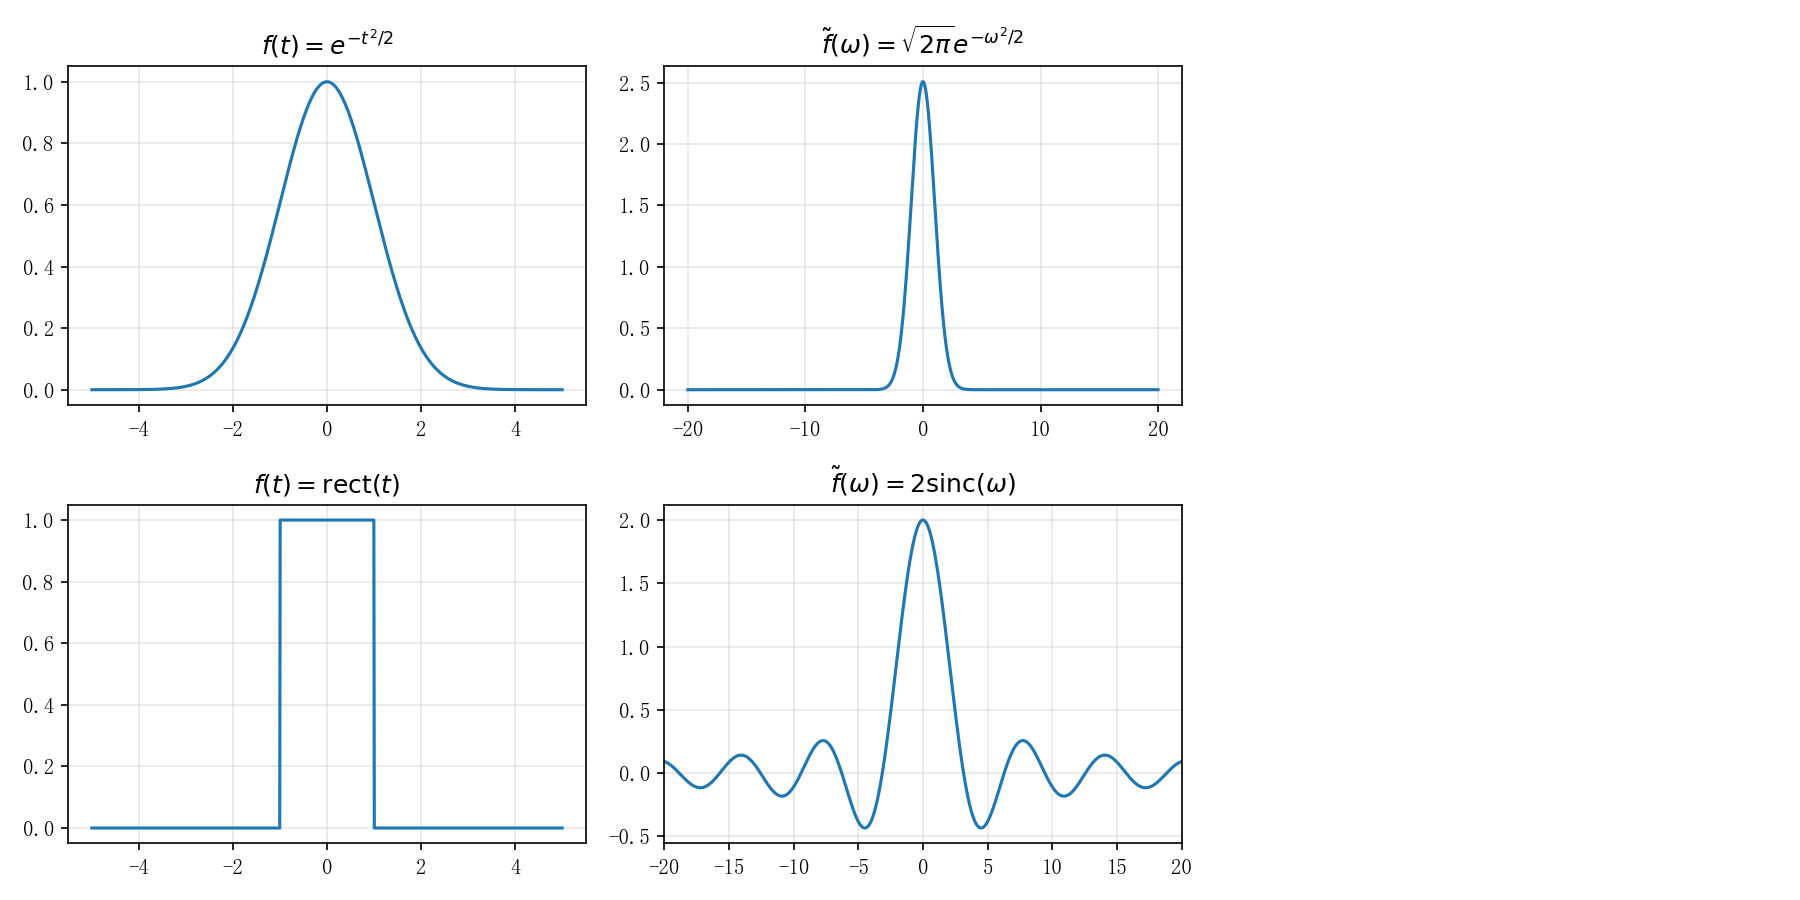
\includegraphics[width=0.85\textwidth]{figures/fig3_2_ft_pairs.png}
\caption{傅里叶变换对示例。上：高斯函数的傅里叶变换仍是高斯。下：矩形脉冲的傅里叶变换是 sinc 函数。注意"窄的时域信号 $\to$ 宽的频域信号"这一对偶性。}
\label{fig:ft_pairs}
\end{figure}

\section{傅里叶变换的物理应用}
\label{sec:ft_physics}

\subsection{衍射与傅里叶光学}

夫琅禾费衍射的光强分布正是孔径函数的傅里叶变换的模平方。单缝衍射：
\begin{equation}
I(\theta) = I_0\,\mathrm{sinc}^2\!\left(\frac{\pi a\sin\theta}{\lambda}\right),
\qquad \mathrm{sinc}\,x = \frac{\sin x}{x}.
\end{equation}

这并非巧合：\textbf{远程衍射图案 = 孔径函数的二维傅里叶变换}。透镜本身就是一个光学傅里叶变换器——物平面和像平面互为傅里叶共轭面。这就是\textbf{傅里叶光学}的核心思想。

\begin{example}[双缝衍射]
双缝间距 $d$，缝宽 $a$。孔径函数是两个矩形函数的卷积：$p_a(x) * [\delta(x-d/2) + \delta(x+d/2)]$。

衍射图案是缝宽衍射和缝间干涉的乘积：
\begin{equation}
I(\theta) = I_0\,\mathrm{sinc}^2\!\left(\frac{\pi a\sin\theta}{\lambda}\right)
\cdot \cos^2\!\left(\frac{\pi d\sin\theta}{\lambda}\right).
\end{equation}

从傅里叶变换角度看：$\mathcal{F}[p_a(x)] \propto \mathrm{sinc}$（单个缝的衍射），$\mathcal{F}[\delta(x-d/2)+\delta(x+d/2)] \propto \cos$（双缝干涉）。卷积的 FT = FT 的乘积，所以衍射图案是两者的乘积！
\end{example}

\begin{insight}
物理光学中最令人惊叹的对应关系：
\begin{itemize}
\item 窄狭缝 $\to$ 宽的衍射图案（窄时域 $\to$ 宽频域）
\item 双缝 $\to$ 双光束干涉（两个 $\delta$ 函数的傅里叶变换是余弦条纹）
\item 光栅 $\to$ 分立谱线（周期结构的变换是离散谱）
\end{itemize}
每一种衍射现象都可以从傅里叶变换的角度获得更深刻的理解。
\end{insight}

\subsection{采样定理与信号处理}

\textbf{采样定理 (Nyquist-Shannon)}：若 $f(t)$ 的最高频率成分为 $f_{\max}$，则采样频率必须 $\geq 2f_{\max}$ 才能无失真地重建原信号。这是模拟-数字转换的基础。

\textbf{证明思路：} 设 $f(t)$ 的频谱在 $|\omega| > \Omega$ 时为零（即带限信号）。以间隔 $T = \pi/\Omega$ 采样得到 $f_s(t) = f(t)\sum_{n=-\infty}^{\infty}\delta(t-nT)$。

采样信号的频谱是原频谱的周期延拓：
\begin{equation}
\tilde{f}_s(\omega) = \frac{1}{T}\sum_{n=-\infty}^{\infty} \tilde{f}(\omega - n\omega_s),\quad \omega_s = \frac{2\pi}{T}.
\end{equation}

只要 $\omega_s \geq 2\Omega$（即 $T \leq \pi/\Omega$），频谱不会混叠，可以通过低通滤波器完美恢复原信号。

\textbf{重建公式：}
\begin{equation}
f(t) = \sum_{n=-\infty}^{\infty} f(nT)\,\mathrm{sinc}\!\left(\frac{\pi t}{T} - n\pi\right).
\end{equation}

\textbf{滤波器设计：} 在频域中设计滤波器是直观的——保留需要的频率成分，抑制不需要的。理想低通滤波器的时域响应是 $\mathrm{sinc}$ 函数，这正是傅里叶变换对 $(\text{矩形窗} \leftrightarrow \text{sinc})$ 的体现。

% FFT 示例图
\begin{figure}[H]
\centering
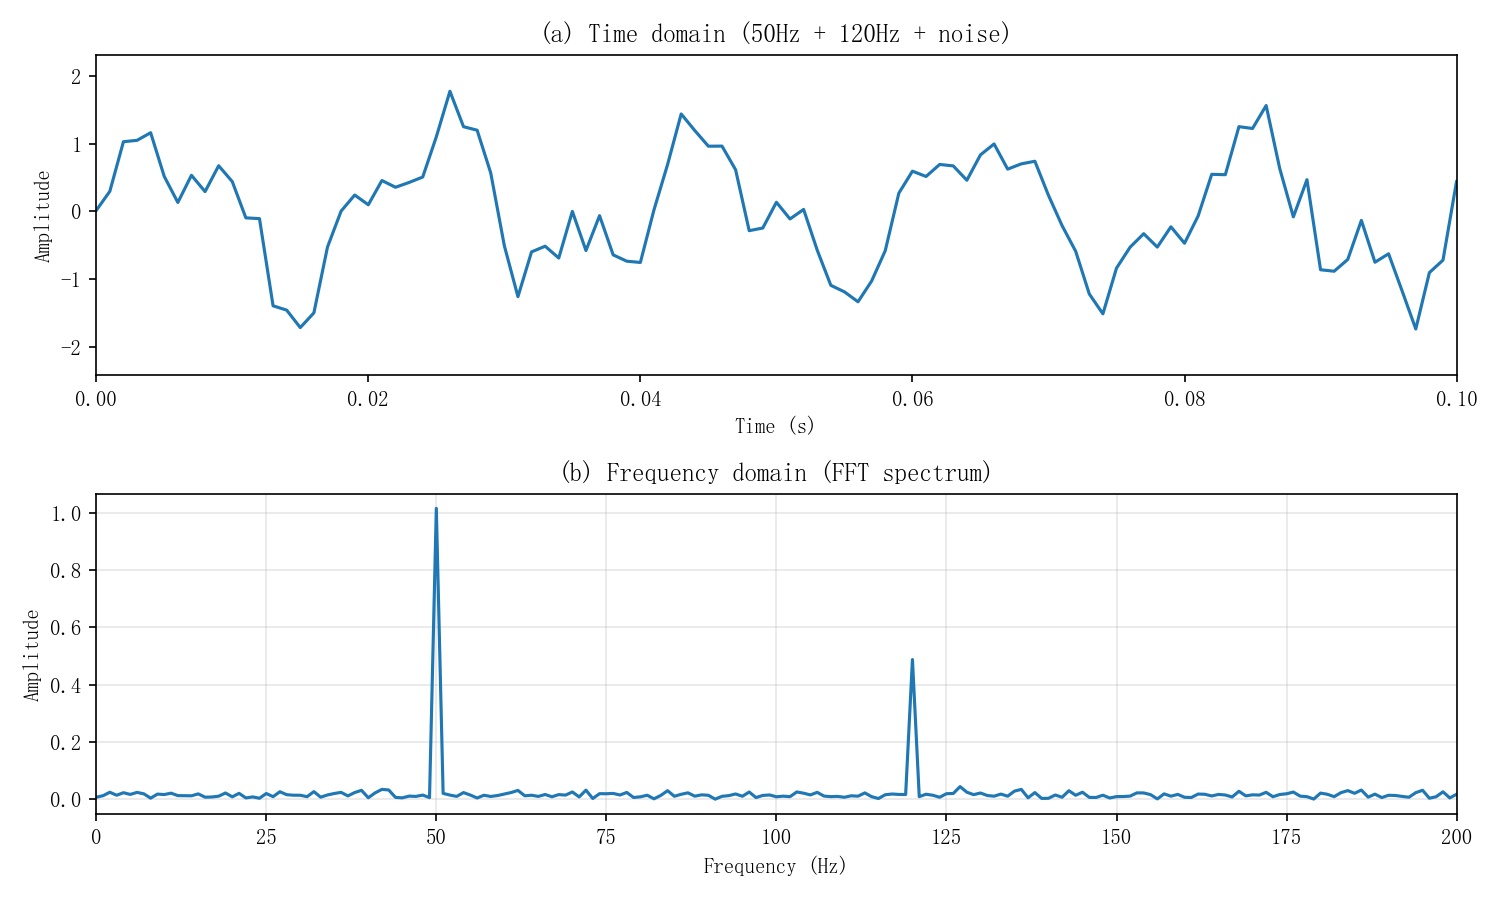
\includegraphics[width=0.8\textwidth]{figures/fig3_3_fft_example.png}
\caption{FFT 频谱分析示例。上：包含 50 Hz 正弦、120 Hz 正弦和噪声的时域信号。下：FFT 振幅谱，50 Hz 和 120 Hz 处清晰可见的峰值。}
\label{fig:fft_example}
\end{figure}

\subsection{量子力学中的动量空间}

波函数在坐标表象和动量表象之间通过傅里叶变换相联系：
\begin{equation}
\tilde{\psi}(p) = \frac{1}{\sqrt{2\pi\hbar}}\int_{-\infty}^{\infty}
\psi(x)\,e^{-\mathrm{i}px/\hbar}\,\dd x.
\end{equation}

动量算符 $\hat{p} = -\mathrm{i}\hbar\partial_x$ 在动量表象中变为乘法算符 $\hat{p} = p$。傅里叶变换在此完成了\textbf{表象变换}的功能——这正是量子力学的数学框架的核心。

\subsection{不确定性原理}

傅里叶变换的时宽-带宽积约束直接导致量子力学中的不确定性原理。

定义时宽 $\Delta t$ 和频宽 $\Delta\omega$：
\begin{align}
(\Delta t)^2 &= \frac{\int (t - \langle t\rangle)^2 |f(t)|^2\,\dd t}{\int |f(t)|^2\,\dd t},\\
(\Delta\omega)^2 &= \frac{\int (\omega - \langle\omega\rangle)^2 |\tilde{f}(\omega)|^2\,\dd\omega}{\int |\tilde{f}(\omega)|^2\,\dd\omega}.
\end{align}

可以证明 $\Delta t \cdot \Delta\omega \geq 1/2$。将 $\omega = p/\hbar$ 代入，得 $\Delta x \cdot \Delta p \geq \hbar/2$。

\textbf{证明（概要）：} 利用施瓦兹不等式：
\begin{align}
\left(\int |f|^2\,\dd t\right)^2
&\leq \int |t f(t)|^2\,\dd t \cdot \int |f'(t)|^2\,\dd t \\
&\leq \Delta t^2 \cdot (\Delta\omega)^2 \cdot \left(\int |f|^2\,\dd t\right)^2.
\end{align}

等号当且仅当 $f(t) \propto e^{-at^2}$（高斯函数）时成立——这正是最小不确定波包。

\subsection{帕塞瓦尔定理与能量守恒}

帕塞瓦尔定理的物理形式：
\begin{equation}
\int_{-\infty}^{\infty} |f(t)|^2\,\dd t
= \frac{1}{2\pi}\int_{-\infty}^{\infty} |\tilde{f}(\omega)|^2\,\dd\omega.
\label{eq:parseval}
\end{equation}

在电学中，左端是信号在时域的总能量，右端是各频率成分的能量之和。能量守恒要求在时域和频域中一致——帕塞瓦尔定理正是这一要求的数学保证。

\subsection{希尔伯特变换与解析信号}

对于实信号 $f(t)$，定义其\textbf{希尔伯特变换}：
\begin{equation}
\hat{f}(t) = \frac{1}{\pi}\mathcal{P}\int_{-\infty}^{\infty} \frac{f(\tau)}{t-\tau}\,\dd\tau.
\end{equation}

在频域中，希尔伯特变换等价于相位移动 $\pm\pi/2$：$\mathcal{F}[\hat{f}](\omega) = -\mathrm{i}\,\mathrm{sgn}(\omega)\tilde{f}(\omega)$。

\textbf{解析信号：} $f_a(t) = f(t) + \mathrm{i}\hat{f}(t)$ 是频域中仅含正频率成分的信号。解析信号在通信理论中用于：
\begin{itemize}
\item 提取瞬时幅度和瞬时相位：$A(t) = |f_a(t)|$, $\phi(t) = \arg f_a(t)$。
\item 定义瞬时频率：$\omega(t) = \phi'(t)$。
\item 单边带调制（SSB）。
\end{itemize}

\section{拉普拉斯变换}
\label{sec:laplace}

\subsection*{动机：傅里叶变换做不到的事情}

傅里叶变换要求函数绝对可积——这对 $e^{t}$、常数函数、甚至 $t^n$ 都不成立。更关键的是，傅里叶变换不自然处理初始条件。拉普拉斯变换通过引入衰减因子 $e^{-\sigma t}$ 解决了这两个问题。

\subsection{从傅里叶到拉普拉斯}

傅里叶变换要求函数在 $\pm\infty$ 绝对可积，许多重要函数（如 $e^{\alpha t}\Theta(t)$ 当 $\alpha>0$、常数函数、多项式）不满足这一条件。引入衰减因子 $e^{-\sigma t}$（$\sigma>0$）迫使积分收敛：
\begin{equation}
\mathcal{L}[f(t)] = F(s)
= \int_0^{\infty} f(t)\,e^{-st}\,\dd t,\qquad s = \sigma + \mathrm{i}\omega.
\label{eq:laplace_transform}
\end{equation}

这是\textbf{单边拉普拉斯变换}，积分下限 $0^-$ 包含原点处的奇异性。相比傅里叶变换，拉普拉斯变换有两个优势：
\begin{itemize}
\item 收敛范围更广（通过 $\sigma$ 控制）。
\item 自然处理初始条件——这是求解初值问题的关键。
\end{itemize}

\subsection{收敛域 (ROC)}

拉普拉斯变换的收敛域是复 $s$ 平面上使得积分收敛的 $\sigma$ 的范围。对于因果信号 $f(t)\Theta(t)$，ROC 是某个 $\sigma > \sigma_c$ 的半平面。

\begin{example}[完整算例：$e^{at}\Theta(t)$ 的拉普拉斯变换]
计算 $\mathcal{L}[e^{at}\Theta(t)]$，$a$ 为实数。

\textbf{步骤 1：写出定义式。}
\begin{equation}
F(s) = \int_0^{\infty} e^{at} e^{-st}\,\dd t
= \int_0^{\infty} e^{-(s-a)t}\,\dd t.
\end{equation}

\textbf{步骤 2：判断收敛性。}
令 $s = \sigma + \mathrm{i}\omega$，$e^{-(s-a)t} = e^{-(\sigma-a)t}e^{-\mathrm{i}\omega t}$。
积分收敛当且仅当 $\sigma - a > 0$，即 $\Re(s) > a$。

\textbf{步骤 3：计算积分。}
当 $\Re(s) > a$ 时：
\begin{equation}
F(s) = \int_0^{\infty} e^{-(s-a)t}\,\dd t
= \left[-\frac{e^{-(s-a)t}}{s-a}\right]_0^{\infty}
= \frac{1}{s-a}.
\end{equation}

\textbf{结论：}
\begin{equation}
\boxed{\;\mathcal{L}[e^{at}\Theta(t)] = \frac{1}{s-a},\quad \Re(s) > a\;}.
\end{equation}
特例：$a=0$ 时 $\mathcal{L}[\Theta(t)] = 1/s$，$\Re(s) > 0$。
\end{example}

\begin{example}[{$\mathcal{L}[\sin(\omega_0 t)\Theta(t)]$} 的推导]
利用欧拉公式 $\sin(\omega_0 t) = (e^{\mathrm{i}\omega_0 t} - e^{-\mathrm{i}\omega_0 t})/(2\mathrm{i})$：
\begin{align*}
\mathcal{L}[\sin(\omega_0 t)\Theta(t)]
&= \frac{1}{2\mathrm{i}}\left[\frac{1}{s-\mathrm{i}\omega_0} - \frac{1}{s+\mathrm{i}\omega_0}\right] \\
&= \frac{1}{2\mathrm{i}}\frac{s+\mathrm{i}\omega_0 - s + \mathrm{i}\omega_0}{s^2 + \omega_0^2}
= \frac{\omega_0}{s^2 + \omega_0^2}.
\end{align*}
ROC: $\Re(s) > 0$。类似可得 $\mathcal{L}[\cos(\omega_0 t)\Theta(t)] = s/(s^2+\omega_0^2)$。
\end{example}

\subsection{拉普拉斯变换的基本性质}

\begin{table}[h]
\centering
\caption{拉普拉斯变换的基本性质}
\label{tab:lt_properties}
\begin{tabular}{c|c}
\toprule
性质 & 变换对 \\
\midrule
时域微分 & $\mathcal{L}[f'(t)] = sF(s) - f(0^-)$ \\
二阶微分 & $\mathcal{L}[f''(t)] = s^2F(s) - sf(0^-) - f'(0^-)$ \\
时域积分 & $\mathcal{L}[\int_0^t f(\tau)\,\dd\tau] = F(s)/s$ \\
频移 & $\mathcal{L}[e^{at}f(t)] = F(s-a)$ \\
时移 & $\mathcal{L}[f(t-a)\Theta(t-a)] = e^{-as}F(s)$ \\
卷积 & $\mathcal{L}[(f*g)(t)] = F(s)G(s)$ \\
初值定理 & $\lim_{t\to0^+} f(t) = \lim_{s\to\infty} sF(s)$ \\
终值定理 & $\lim_{t\to\infty} f(t) = \lim_{s\to0} sF(s)$（极点均在左半平面） \\
\bottomrule
\end{tabular}
\end{table}

\textbf{时域微分性质}是拉普拉斯变换求解 ODE 的关键——它将微分方程转化为代数方程，同时自动引入初始条件。

\begin{proof}[二阶微分性质的推导]
先应用一次微分性质：
\begin{align*}
\mathcal{L}[f''(t)] &= s\mathcal{L}[f'(t)] - f'(0^-) \\
&= s[sF(s) - f(0^-)] - f'(0^-) \\
&= s^2F(s) - sf(0^-) - f'(0^-).
\end{align*}
依此类推，$n$ 阶导数的拉普拉斯变换为：
\begin{equation}
\mathcal{L}[f^{(n)}(t)] = s^nF(s) - s^{n-1}f(0^-) - \cdots - f^{(n-1)}(0^-).
\end{equation}
\end{proof}

\subsection{逆变换与部分分式展开法}

拉普拉斯逆变换的公式为：
\begin{equation}
f(t) = \frac{1}{2\pi\mathrm{i}}\int_{\sigma_0-\mathrm{i}\infty}^{\sigma_0+\mathrm{i}\infty}
F(s)\,e^{st}\,\dd s,
\label{eq:inverse_laplace}
\end{equation}
其中 $\sigma_0$ 位于 ROC 内。该积分可以用留数定理计算。

\textbf{部分分式展开法} 是工程中更常用的方法：将 $F(s)$ 分解为低阶项之和，查表得逆变换。

\begin{example}[部分分式展开的通用方法]
设 $F(s) = \frac{N(s)}{D(s)}$，分母次数高于分子次数。

\textbf{情况 1：所有根为单根。}
$D(s) = (s-p_1)(s-p_2)\cdots(s-p_n)$。
\begin{equation}
\frac{N(s)}{D(s)} = \sum_{k=1}^n \frac{A_k}{s-p_k},\quad
A_k = \lim_{s\to p_k} (s-p_k)\frac{N(s)}{D(s)}.
\end{equation}

\textbf{情况 2：有重根。}
若 $p_1$ 是 $m$ 重根：
\begin{equation}
\frac{N(s)}{(s-p_1)^m\cdots} = \frac{A_{1,m}}{(s-p_1)^m} + \frac{A_{1,m-1}}{(s-p_1)^{m-1}} + \cdots + \frac{A_{1,1}}{s-p_1} + \cdots,
\end{equation}
其中 $A_{1,k} = \frac{1}{(k-1)!}\lim_{s\to p_1}\frac{\dd^{k-1}}{\dd s^{k-1}}\left[(s-p_1)^m\frac{N(s)}{D(s)}\right]$。

\textbf{情况 3：共轭复根。}
保留为二次项形式 $\frac{As+B}{(s+\alpha)^2+\beta^2}$，对应时域中的衰减正弦/余弦。
\end{example}

\begin{example}[完整算例：用拉普拉斯变换解一阶微分方程]
求解 $y' + 2y = e^{-t}$，$y(0)=1$。

\textbf{步骤 1：两边做拉普拉斯变换。}
$\mathcal{L}[y'] + 2\mathcal{L}[y] = \mathcal{L}[e^{-t}]$。
$sY(s) - y(0) + 2Y(s) = \frac{1}{s+1}$。

\textbf{步骤 2：代入初始条件。}
$sY(s) - 1 + 2Y(s) = \frac{1}{s+1}$。
$(s+2)Y(s) = 1 + \frac{1}{s+1}$。

\textbf{步骤 3：解出 $Y(s)$。}
\begin{align*}
Y(s) &= \frac{1}{s+2} + \frac{1}{(s+1)(s+2)} \\
&= \frac{1}{s+2} + \left(\frac{1}{s+1} - \frac{1}{s+2}\right) \\
&= \frac{1}{s+1}.
\end{align*}
（部分分式展开：$\frac{1}{(s+1)(s+2)} = \frac{A}{s+1} + \frac{B}{s+2}$，解得 $A=1,B=-1$。）

\textbf{步骤 4：逆变换。}
$y(t) = \mathcal{L}^{-1}\left[\frac{1}{s+1}\right] = e^{-t}$。

\textbf{验证：} $y' = -e^{-t}$，$y'+2y = -e^{-t}+2e^{-t}=e^{-t}$，$y(0)=1$。正确！
\end{example}

\begin{example}[完整算例：二阶 ODE——受迫阻尼振荡]
求解 $y'' + 2y' + 5y = 10\sin t$，$y(0)=0$, $y'(0)=0$。

\textbf{步骤 1：拉普拉斯变换。}
$[s^2Y(s) - 0 - 0] + 2[sY(s) - 0] + 5Y(s) = 10\cdot\frac{1}{s^2+1}$。
$(s^2 + 2s + 5)Y(s) = \frac{10}{s^2+1}$。

\textbf{步骤 2：解出 $Y(s)$。}
\begin{equation}
Y(s) = \frac{10}{(s^2+2s+5)(s^2+1)}.
\end{equation}

\textbf{步骤 3：部分分式展开。}
设：
\begin{equation}
\frac{10}{(s^2+2s+5)(s^2+1)} = \frac{As+B}{s^2+2s+5} + \frac{Cs+D}{s^2+1}.
\end{equation}
通分后比较系数：
\begin{align*}
A + C &= 0,\\
B + 2C + D &= 0,\\
A + 2D + 5C &= 0,\\
B + 5D &= 10.
\end{align*}
解得 $A = -\frac{5}{4}$, $B = \frac{5}{4}$, $C = \frac{5}{4}$, $D = \frac{15}{4}$。

因此：
\begin{equation}
Y(s) = \frac{-\frac{5}{4}s + \frac{5}{4}}{(s+1)^2 + 2^2} + \frac{\frac{5}{4}s + \frac{15}{4}}{s^2+1}.
\end{equation}

\textbf{步骤 4：逆变换（查表）。}
\begin{align*}
y(t) &= -\frac{5}{4}e^{-t}\cos 2t + \frac{5}{2}e^{-t}\sin 2t + \frac{5}{4}\cos t + \frac{15}{4}\sin t.
\end{align*}

前两项是瞬态解（指数衰减），后两项是稳态解（持续振荡）。
\end{example}

% ROC 示意图
\begin{figure}[H]
\centering
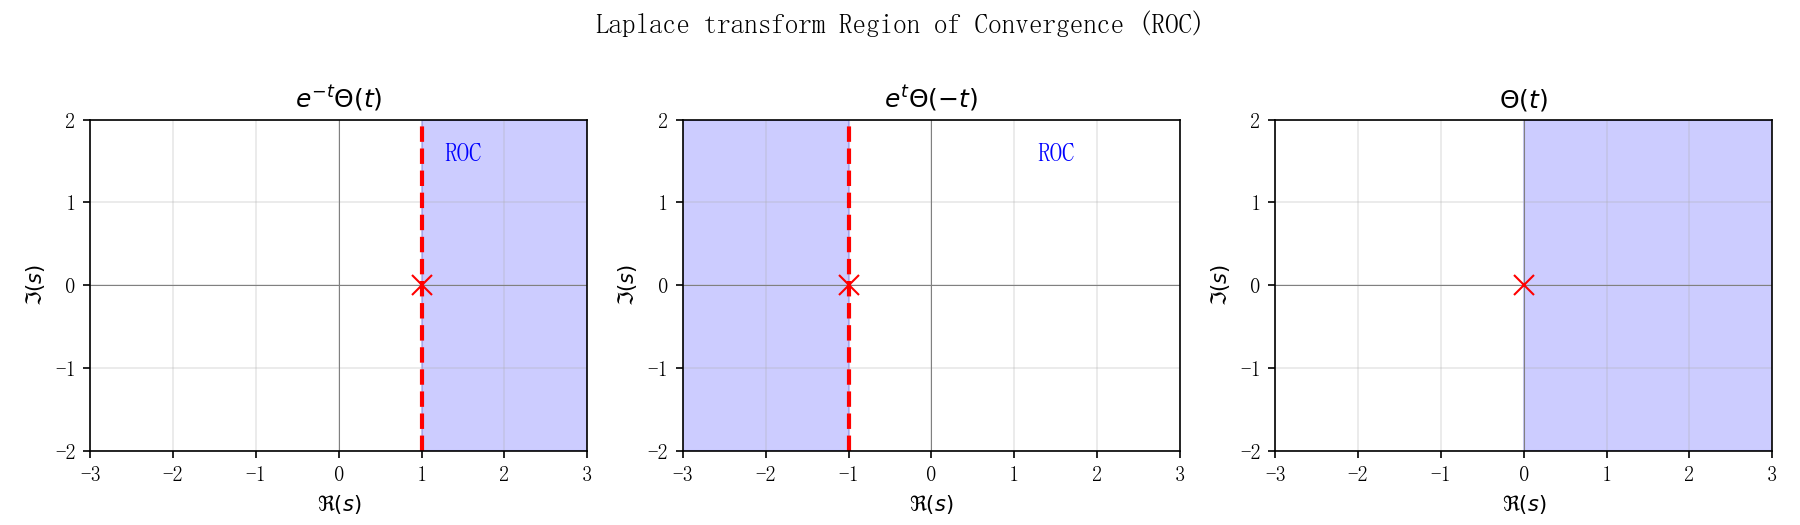
\includegraphics[width=0.85\textwidth]{figures/fig3_4_laplace_roc.png}
\caption{拉普拉斯变换的收敛域 (ROC)。左：$e^{-t}\Theta(t)$ 的 ROC 为 $\Re(s) > -1$；中：$e^{t}\Theta(-t)$（左信号）的 ROC 为 $\Re(s) < 1$；右：$\Theta(t)$ 的 ROC 为 $\Re(s) > 0$。}
\label{fig:laplace_roc}
\end{figure}

\section{拉普拉斯变换的物理应用}
\label{sec:laplace_physics}

\subsection{电路的复频域分析}

\textbf{阻抗法：} 在 $s$ 域中，电感 $L$ 的阻抗为 $sL$，电容 $C$ 的阻抗为 $1/(sC)$，电阻 $R$ 的阻抗为 $R$。这与相量法中的 $\mathrm{i}\omega L$, $1/(\mathrm{i}\omega C)$ 形式一致，但 $s$ 域方法可以处理非正弦激励和初始条件。

\textbf{传递函数：} 系统的输出-输入比 $H(s) = Y(s)/X(s)$ 称为\textbf{传递函数}。它是系统的频域指纹，完全刻画了系统的线性响应特性。
\begin{itemize}
\item 系统的稳定性等价于 $H(s)$ 的所有极点具有负实部。
\item 单位冲激响应 $h(t) = \mathcal{L}^{-1}[H(s)]$。
\item 阶跃响应 $s(t) = \mathcal{L}^{-1}[H(s)/s]$。
\end{itemize}

\begin{example}[完整算例：RLC 电路的阶跃响应]
设串联 RLC 电路初始电流为零，电容初始电压为零。在 $t=0$ 时施加阶跃电压 $V_0\Theta(t)$。

\textbf{步骤 1：写出复频域阻抗。}
$Z(s) = sL + R + 1/(sC)$。

\textbf{步骤 2：电流的拉普拉斯变换。}
\begin{align*}
I(s) &= \frac{V_0/s}{Z(s)} = \frac{V_0}{s(sL + R + 1/(sC))} \\
&= V_0\frac{C}{s^2 LC + sRC + 1}
= \frac{V_0/L}{s^2 + (R/L)s + 1/(LC)}.
\end{align*}

\textbf{步骤 3：引入标准参数。}
令 $\alpha = R/(2L)$（衰减系数），$\omega_0 = 1/\sqrt{LC}$（谐振频率）。
则 $I(s) = \frac{V_0/L}{s^2 + 2\alpha s + \omega_0^2}$。

\textbf{步骤 4：分情况逆变换。}

\underline{欠阻尼 ($\alpha<\omega_0$)：}
令 $\omega_d = \sqrt{\omega_0^2 - \alpha^2}$（阻尼谐振频率）。
\begin{align*}
I(s) &= \frac{V_0/L}{(s+\alpha)^2 + \omega_d^2}, \\
i(t) &= \frac{V_0}{\omega_d L}e^{-\alpha t}\sin(\omega_d t)\,\Theta(t).
\end{align*}

\underline{临界阻尼 ($\alpha=\omega_0$)：}
$I(s) = \frac{V_0/L}{(s+\alpha)^2}$，
$i(t) = \frac{V_0}{L}t e^{-\alpha t}\Theta(t)$。

\underline{过阻尼 ($\alpha>\omega_0$)：}
令 $\beta_{1,2} = \alpha \pm \sqrt{\alpha^2 - \omega_0^2}$。
\begin{align*}
I(s) &= \frac{V_0/L}{(s+\beta_1)(s+\beta_2)}, \\
i(t) &= \frac{V_0}{L(\beta_1-\beta_2)}\left(e^{-\beta_2 t} - e^{-\beta_1 t}\right)\Theta(t).
\end{align*}

拉普拉斯变换将二阶微分方程的初值问题化为代数方程求解，再通过逆变换返回时域。这是求解线性系统的标准方法。
\end{example}

\subsection{传递函数与稳定性分析}

传递函数 $H(s)$ 的极点位置决定系统稳定性：
\begin{itemize}
\item 所有极点在左半平面 $\to$ 稳定（瞬态解指数衰减）。
\item 任何极点在右半平面 $\to$ 不稳定（瞬态解指数增长）。
\item 极点在虚轴上（单根）$\to$ 临界稳定（无阻尼振荡）。
\end{itemize}

\textbf{伯德图 (Bode plot)} 是传递函数 $H(\mathrm{i}\omega)$ 的幅频和相频曲线，采用对数坐标。它直观显示了系统对不同频率输入的响应特性。

\begin{example}[一阶低通滤波器的伯德图]
$H(s) = \frac{1}{1 + sRC}$。

幅频响应（dB）：
\begin{equation}
|H(\mathrm{i}\omega)|_{\text{dB}} = -10\log_{10}\left[1 + (\omega RC)^2\right].
\end{equation}
\begin{itemize}
\item $\omega \ll 1/(RC)$：$|H|_{\text{dB}} \approx 0$ dB（通带）。
\item $\omega \gg 1/(RC)$：$|H|_{\text{dB}} \approx -20\log_{10}(\omega RC)$ dB/十倍频（阻带，斜率 $-20$ dB/dec）。
\item $\omega = 1/(RC)$（截止频率）：$|H|_{\text{dB}} = -3$ dB。
\end{itemize}

相频响应：
\begin{equation}
\angle H(\mathrm{i}\omega) = -\arctan(\omega RC).
\end{equation}
在截止频率处，相位滞后 $45^\circ$。
\end{example}

\subsection{力学系统的类比}

机械振动系统（质量-弹簧-阻尼）与 RLC 电路通过拉普拉斯变换展示出完美的\textbf{力-电类比}：
\begin{equation}
\text{力学：}\quad M s^2 + B s + K \quad\longleftrightarrow\quad
\text{电路：}\quad L s^2 + R s + \frac{1}{C}.
\end{equation}

\begin{table}[h]
\centering
\caption{力-电类比}
\label{tab:mech_elect_analogy}
\begin{tabular}{c|c}
\toprule
力学系统 & 电路系统 \\
\midrule
质量 $M$ & 电感 $L$ \\
阻尼系数 $B$ & 电阻 $R$ \\
劲度系数 $K$ & 倒数电容 $1/C$ \\
力 $F$ & 电压 $V$ \\
速度 $v$ & 电流 $I$ \\
动量 $p$ & 磁通 $\Phi$ \\
\bottomrule
\end{tabular}
\end{table}

\begin{insight}
力-电类比不是肤浅的形式相似，而是源于相同的数学模型。任何一个二阶线性系统——不论是机械的、电气的、声学的还是热学的——都可以用传递函数统一处理。这种 \textbf{跨领域统一性} 是物理学家追求的最高境界。拉普拉斯变换通过揭示不同物理系统中相同的数学结构，实现了这种统一。
\end{insight}

\subsection{偏微分方程中的应用}

考虑半无限长杆的热传导方程：
\begin{equation}
\frac{\partial u}{\partial t} = \kappa \frac{\partial^2 u}{\partial x^2},\quad
x>0,\; t>0,
\end{equation}
初始条件 $u(x,0)=0$，边界条件 $u(0,t)=u_0$，$u(\infty,t)=0$。

对 $t$ 做拉普拉斯变换，偏微分方程化为常微分方程：
\begin{equation}
sU(x,s) = \kappa \frac{\dd^2 U}{\dd x^2}.
\end{equation}

解得 $U(x,s) = C(s)e^{-x\sqrt{s/\kappa}}$。代入边界条件得 $C(s) = u_0/s$，于是
\begin{equation}
U(x,s) = \frac{u_0}{s}e^{-x\sqrt{s/\kappa}}.
\end{equation}

查逆变换表或利用留数定理：
\begin{equation}
u(x,t) = u_0\,\mathrm{erfc}\!\left(\frac{x}{2\sqrt{\kappa t}}\right),
\quad \mathrm{erfc}(z) = \frac{2}{\sqrt{\pi}}\int_z^{\infty} e^{-\eta^2}\,\dd\eta.
\label{eq:heat_laplace_sol}
\end{equation}

\textbf{物理信息：} 温度扰动传播的大致距离为 $\sqrt{\kappa t}$——这正是扩散长度。拉普拉斯变换如此自然地给出了这个重要标度律。

\section*{拉普拉斯变换表}

\begin{table}[h]
\centering
\caption{常用拉普拉斯变换对}
\label{tab:laplace_table}
\begin{tabular}{c|c}
\toprule
$f(t)$ ($t\geq0$) & $F(s) = \mathcal{L}[f]$ \\
\midrule
$\delta(t)$ & $1$ \\
$\Theta(t)$ & $1/s$ \\
$t$ & $1/s^2$ \\
$t^n$ & $n!/s^{n+1}$ \\
$e^{at}$ & $1/(s-a)$ \\
$\sin(\omega_0 t)$ & $\omega_0/(s^2+\omega_0^2)$ \\
$\cos(\omega_0 t)$ & $s/(s^2+\omega_0^2)$ \\
$e^{at}\sin(\omega_0 t)$ & $\omega_0/[(s-a)^2+\omega_0^2]$ \\
$e^{at}\cos(\omega_0 t)$ & $(s-a)/[(s-a)^2+\omega_0^2]$ \\
$t e^{at}$ & $1/(s-a)^2$ \\
$t^n e^{at}$ & $n!/(s-a)^{n+1}$ \\
$\sinh(at)$ & $a/(s^2-a^2)$ \\
$\cosh(at)$ & $s/(s^2-a^2)$ \\
\bottomrule
\end{tabular}
\end{table}

\section{傅里叶变换与拉普拉斯变换的比较}

\begin{table}[h]
\centering
\caption{傅里叶变换与拉普拉斯变换对比}
\label{tab:ft_vs_lt}
\begin{tabular}{c|c}
\toprule
傅里叶变换 & 拉普拉斯变换 \\
\midrule
$s = \mathrm{i}\omega$（纯虚频率） & $s = \sigma + \mathrm{i}\omega$（复频率） \\
双侧变换（$-\infty\to\infty$） & 单侧变换（$0\to\infty$） \\
需要绝对可积条件 & 收敛域更广 \\
稳态分析 & 暂态+稳态 \\
频谱分析 & 传递函数与稳定性 \\
不能处理初始条件 & 自然包含初始条件 \\
\bottomrule
\end{tabular}
\end{table}

\textbf{选择指南：}
\begin{itemize}
\item 分析稳态周期信号、频谱结构、光学衍射 $\to$ 傅里叶变换。
\item 求解初值问题、暂态响应、系统稳定性 $\to$ 拉普拉斯变换。
\item 两者通过 $s = \sigma + \mathrm{i}\omega$ 相联系：傅里叶变换是拉普拉斯变换在虚轴上的特例（当 ROC 包含虚轴时）。
\end{itemize}

\section{本章小结}

\begin{itemize}
\item \textbf{傅里叶级数} 将周期函数分解为离散谐波，是频域分析的起点。
\item \textbf{傅里叶变换} 将时域与频域通过积分变换精确对应，揭示了时频对偶性。
\item \textbf{傅里叶变换的卷积定理} 表明时域卷积对应于频域乘法，这是线性系统分析的基石。
\item \textbf{采样定理} 给出了数字信号处理中采样率的理论下限。
\item \textbf{拉普拉斯变换} 推广了傅里叶变换，通过复频率 $s$ 处理更广泛的函数和初始条件。
\item \textbf{传递函数} 是系统的频域特征函数，稳定性由极点位置决定。
\item \textbf{两个变换统一} 了力学、电学、热学、光学中的线性分析。
\end{itemize}

\subsection*{概念图谱}

\begin{center}
\fbox{\parbox{0.92\textwidth}{
\textbf{积分变换的概念网络：}\\[3pt]
$\bullet$ 周期信号 $\to$ 傅里叶级数（三角形式 $\leftrightarrow$ 复数形式）\\[3pt]
$\bullet$ 傅里叶级数 $\xrightarrow{T\to\infty}$ 傅里叶变换 $\to$ 频谱分析 / 衍射 / 量子力学\\[3pt]
$\bullet$ 卷积定理 $\to$ 线性系统：输出 = 输入 $*$ 冲激响应\\[3pt]
$\bullet$ 采样定理 $\to$ 数字信号处理的基础\\[3pt]
$\bullet$ 傅里叶变换 $\xrightarrow{\text{收敛因子}}$ 拉普拉斯变换 $\to$ ODE/PDE 求解\\[3pt]
$\bullet$ 传递函数 $H(s)$ $\to$ 稳定性分析 / 伯德图 / 滤波器设计\\[3pt]
$\bullet$ Kramers-Kronig 关系：因果性 + 解析性的物理推论
}}
\end{center}

\subsection*{公式参考表}

\begin{table}[h]
\centering
\caption{积分变换核心公式速查}
\label{tab:transform_formulas}
\begin{tabular}{c|c}
\toprule
公式 & 说明 \\
\midrule
$c_n = \frac{1}{T}\int_{-T/2}^{T/2} f(t)e^{-\mathrm{i}n\omega_0 t}\,\dd t$ & 傅里叶级数系数 \\
$\tilde{f}(\omega) = \int_{-\infty}^{\infty} f(t)e^{-\mathrm{i}\omega t}\,\dd t$ & 傅里叶正变换 \\
$f(t) = \frac{1}{2\pi}\int_{-\infty}^{\infty} \tilde{f}(\omega)e^{\mathrm{i}\omega t}\,\dd\omega$ & 傅里叶逆变换 \\
$\mathcal{F}[f'(t)] = \mathrm{i}\omega\tilde{f}(\omega)$ & FT 时域微分 \\
$\mathcal{F}[(f*g)(t)] = \tilde{f}(\omega)\tilde{g}(\omega)$ & FT 卷积定理 \\
$\Delta t\,\Delta\omega \geq 1/2$ & 时宽-带宽积 \\
$F(s) = \int_0^{\infty} f(t)e^{-st}\,\dd t$ & 拉普拉斯变换 \\
$\mathcal{L}[f'(t)] = sF(s) - f(0^-)$ & LT 时域微分 \\
$\mathcal{L}[(f*g)(t)] = F(s)G(s)$ & LT 卷积定理 \\
$f(t) = \frac{1}{2\pi\mathrm{i}}\int_{\sigma_0-\mathrm{i}\infty}^{\sigma_0+\mathrm{i}\infty} F(s)e^{st}\,\dd s$ & 拉普拉斯逆变换 \\
\bottomrule
\end{tabular}
\end{table}

\section*{习题}

\textbf{基础题（巩固概念）}

\begin{enumerate}
\item 求周期为 $2\pi$ 的方波 $f(t) = \mathrm{sgn}(\sin t)$ 的傅里叶级数展开（三角形式和复数形式）。
\item 证明傅里叶变换的时移性质：若 $\tilde{f}(\omega) = \mathcal{F}[f(t)]$，则 $\mathcal{F}[f(t-t_0)] = e^{-\mathrm{i}\omega t_0}\tilde{f}(\omega)$。
\item 计算 $\mathcal{F}[e^{-a|t|}]$（$a>0$），并验证帕塞瓦尔定理。
\item 求 $\mathcal{L}[\sin(\omega_0 t)\Theta(t)]$ 和 $\mathcal{L}[\cos(\omega_0 t)\Theta(t)]$。
\item 求矩形脉冲 $p_T(t)$ 的傅里叶变换，并画出 $T=1$ 和 $T=2$ 时的幅度谱 $|\tilde{p}_T(\omega)|$。
\item 求 $\mathcal{L}[t^2 e^{-3t}\Theta(t)]$。
\end{enumerate}

\textbf{提高题（应用分析）}

\begin{enumerate}
\item[7.] 利用傅里叶变换求解一维无限长弦的波动方程 $u_{tt} = c^2 u_{xx}$，初始条件 $u(x,0)=\phi(x)$，$u_t(x,0)=0$。\textbf{提示：} 对 $x$ 做傅里叶变换，求解关于 $t$ 的 ODE，然后逆变换。
\item[8.] 求传递函数 $H(s) = \frac{1}{(s+1)(s+2)}$ 的单位冲激响应和单位阶跃响应。
\item[9.] 用拉普拉斯变换求解 $LC$ 串联电路的零状态响应（施加 $V_0\sin(\omega t)$ 电压）。讨论 $\omega = \omega_0 = 1/\sqrt{LC}$ 时的共振情形。
\item[10.] 求 $f(t) = t^n\Theta(t)$ 的拉普拉斯变换，验证 $\mathcal{L}[t^n] = n!/s^{n+1}$。
\item[11.] 一个二阶低通滤波器 $H(s) = \frac{\omega_0^2}{s^2 + 2\alpha s + \omega_0^2}$。讨论 $\alpha=0$（无阻尼）、$\alpha<\omega_0$（欠阻尼）、$\alpha=\omega_0$（临界阻尼）时的单位阶跃响应，并画出 $h(t)$ 的波形。
\item[12.] 求 $f(t) = \cos(100\pi t)$ 的傅里叶变换。如果以 $f_s=120$ Hz 采样，解释为什么会出现混叠（aliasing）现象。
\end{enumerate}

\textbf{挑战题（综合拓展）}

\begin{enumerate}
\item[13.]（因果性与解析性）因果信号 $f(t)=\Theta(t)\sin(\omega_0 t)e^{-\alpha t}$ 的傅里叶变换是什么？它与拉普拉斯变换有何关系？验证当 $\alpha\to0^+$ 时结果趋近于正弦函数的变换。
\item[14.]（采样定理的证明）设 $f(t)$ 的傅里叶变换在 $|\omega|>\Omega$ 时为零（带限信号）。证明采样定理：$f(t) = \sum_{n=-\infty}^{\infty} f(n\pi/\Omega)\,\mathrm{sinc}(\Omega t - n\pi)$。
\item[15.]（热传导方程的 Laplace 解）用拉普拉斯变换求解有限长杆 $0<x<L$ 的热传导方程，两端温度 $u(0,t)=u(L,t)=0$，初始温度 $u(x,0)=T_0$。对比分离变量法的结果。
\item[16.]（调制与解调）信号 $m(t)$ 被载波 $\cos(\omega_c t)$ 调制为 $f(t)=m(t)\cos(\omega_c t)$。用傅里叶变换解释如何通过低通滤波器从 $f(t)$ 恢复 $m(t)$。
\item[17.]（希尔伯特变换）证明解析信号 $f_a(t) = f(t) + \mathrm{i}\hat{f}(t)$ 的傅里叶变换 $\tilde{f}_a(\omega)$ 在 $\omega<0$ 时为零。利用这个性质解释如何从实信号构造其复包络。
\item[18.]（分数阶傅里叶变换）分数阶傅里叶变换 $F^{\alpha}[f]$ 是传统 FT 的推广。说明当 $\alpha=0$ 时就是恒等变换，$\alpha=\pi/2$ 时是标准傅里叶变换，$\alpha=\pi$ 时是时间反转。讨论其在量子力学中的 chirp 信号分析中的应用。
\end{enumerate}
